\documentclass[aspectratio=169,11pt]{beamer}
\usepackage{booktabs,graphicx,tikz}
\graphicspath{{../Machine_Learning_in_Forex_LaTeX/figures/}}
\definecolor{navy}{HTML}{123450}
\definecolor{accent}{HTML}{00786F}
\setbeamercolor{frametitle}{fg=navy}
\setbeamercolor{structure}{fg=accent}
\setbeamercolor{footline}{fg=navy}
\setbeamertemplate{navigation symbols}{}
\setbeamersize{text margin left=9mm,text margin right=9mm}
\setbeamertemplate{footline}{\hspace{9mm}IIT Indore\quad|\quad Prince Kumar\hfill\insertframenumber\hspace{9mm}\vspace{3mm}}
\newcommand{\key}[1]{\par\medskip{\color{accent}\bfseries #1}\par}
\newcommand{\pair}[3]{\begin{columns}[c,onlytextwidth]\begin{column}{.57\textwidth}\centering\includegraphics[width=\linewidth,height=5.35cm,keepaspectratio]{#1}\end{column}\begin{column}{.39\textwidth}\textbf{#2}\par\medskip #3\end{column}\end{columns}}
\title{Machine Learning for Financial Market Forecasting and Algorithmic Trading}
\author{Prince Kumar}
\begin{document}
\begin{frame}[plain]

\includegraphics[height=1.35cm]{1-IITI_Logo.png}\hfill{\small B.Tech Project $\cdot$ Final Presentation}
\par\bigskip{\LARGE\bfseries\color{navy}\inserttitle\par}
\bigskip Prince Kumar \quad $\cdot$ \quad 230051013\\
Engineering Physics, IIT Indore\\[2mm]
{\small Supervisors: Prof. Raghunath Sahoo and Dr. Kalindi C. Pradhan}
\end{frame}

\begin{frame}{From forecasting currencies to trading portfolios}
\centering
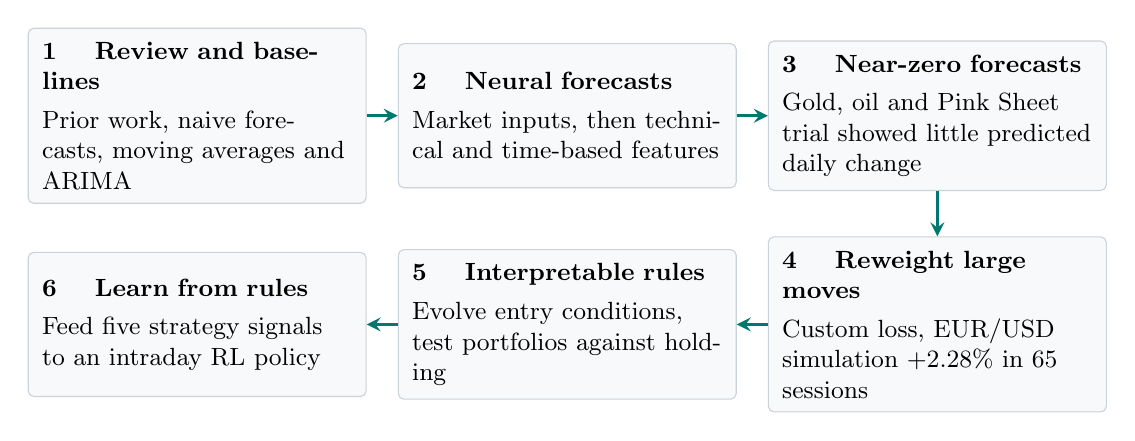
\begin{tikzpicture}[
stage/.style={draw=navy!22,fill=navy!3,rounded corners=2pt,text width=3.94cm,minimum height=1.83cm,align=left,inner sep=5pt,font=\small},
pathway/.style={->,>=stealth,line width=1.2pt,draw=accent}]
\node[stage] (review) at (0,0) {\textbf{1 \quad Review and baselines}\\[3pt]Prior work, naive forecasts, moving averages and ARIMA};
\node[stage] (neural) at (4.7,0) {\textbf{2 \quad Neural forecasts}\\[3pt]Market inputs, then technical and time-based features};
\node[stage] (flat) at (9.4,0) {\textbf{3 \quad Near-zero forecasts}\\[3pt]Gold, oil and Pink Sheet trial showed little predicted daily change};
\node[stage] (loss) at (9.4,-2.65) {\textbf{4 \quad Reweight large moves}\\[3pt]Custom loss, EUR/USD simulation +2.28\% in 65 sessions};
\node[stage] (rules) at (4.7,-2.65) {\textbf{5 \quad Interpretable rules}\\[3pt]Evolve entry conditions, test portfolios against holding};
\node[stage] (agent) at (0,-2.65) {\textbf{6 \quad Learn from rules}\\[3pt]Feed five strategy signals to an intraday RL policy};
\foreach \a/\b in {review/neural,neural/flat,flat/loss,loss/rules,rules/agent} \draw[pathway] (\a) -- (\b);
\end{tikzpicture}
\par\medskip
{\small\color{navy}Best portfolio backtests (cumulative) \textbf{India +250.87\%} (2020--25) \qquad \textbf{US +12.50\%} (2025--26)}
\end{frame}
\begin{frame}{When does a forecast become a profitable trade?}
\begin{columns}[T,onlytextwidth]
\begin{column}{.47\textwidth}
\key{Daily forex}
\textbf{Can a currency forecast guide a trade?}
\begin{enumerate}
\item Predict the next day's exchange rate or return.
\item Compare direction calls with always predicting up.
\item Trade EUR/USD and compare the account with holding euros.
\end{enumerate}
\end{column}
\begin{column}{.47\textwidth}
\key{Intraday equities}
\textbf{Which signals earn a place in a shared portfolio?}
\begin{enumerate}
\item Audit minute bars and test forecast-driven entries.
\item Search for trading rules and evaluate them on later months.
\item Allocate capital across stocks and measure returns after fees.
\end{enumerate}
\end{column}
\end{columns}
\end{frame}

\begin{frame}{USD/INR price errors fell as features were added}
\centering
\begin{tabular}{lrrr}\toprule
Model & Test days & RMSE (INR per USD) & Direction\\\midrule
Base MLP & 690 & 1.9150 & 44.93\%\\
With technical features & 680 & 0.2553 & 52.21\%\\
Technical + temporal features & 675 & 0.2395 & 52.30\%\\\bottomrule
\end{tabular}
\par\bigskip\raggedright Adding temporal features reduced RMSE again, while directional accuracy moved only 0.09 percentage points. The three runs cover slightly different test samples.
\key{The next experiment predicts the daily log return directly.}
\end{frame}

\begin{frame}{How the daily LSTM makes a forecast}
\key{Input and target}
Ten daily observations, each with 23 forex features, predict the next log return, $\log(P_{t+1}/P_t)$.
\key{Training}
A 32-unit LSTM feeds a linear output. Larger realized moves receive more weight in the squared error. The added sign penalty has zero gradient almost everywhere.
\key{Evaluation}
Split observations in time order (80/10/10) and fit scaling on training data. Score the sign of each held-out return, counting flat as up.
\end{frame}

\begin{frame}{What goes into one daily forex forecast?}
\small
Each forecast uses \textbf{10 consecutive days}, with the same \textbf{23 inputs per day}.
\medskip

\begin{tabular}{@{}rlp{9.4cm}@{}}\toprule
Count & Feature group & What the model sees each day\\\midrule
5 & Market data & USD/INR, USD/JPY, EUR/USD, the US federal funds rate and the US 10-year Treasury yield.\\
10 & Trend & Simple and exponential moving averages of the target exchange rate over 5, 10, 30, 50 and 100 days.\\
8 & Momentum and risk & RSI, three Bollinger Band levels, volatility, two average true range proxies (absolute and percentage), and the daily log return.\\\bottomrule
\end{tabular}

\key{What happened when we added commodities?}
In an exploratory run with gold prices, crude oil prices and World Bank Pink Sheet data, the model predicted next-day currency returns close to \textbf{0\%}, even on days when a directional forecast was needed.
\end{frame}
\begin{frame}{USD/INR gained three correct calls over always-up}
\centering
\begin{tabular}{lrrr}\toprule
Currency pair & Always up & LSTM (initial training) & LSTM (after extra training)\\\midrule
USD/INR & 55.07\% & 55.51\% & ---\\
EUR/USD & 50.07\% & 50.95\% & 53.30\%\\\bottomrule
\end{tabular}
\bigskip\raggedright
\key{USD/INR} The model called 378 directions correctly. Predicting up every day already got 375 right.
\key{EUR/USD} We continued training the same LSTM on the validation period. On the same 681 later test days, it called 363 directions correctly, up from 347.
\end{frame}

\begin{frame}{EUR/USD execution changed the size of the gain}
\pair{5-eur-benchmark.png}{65 sessions, 27 July--23 October 2026}{From USD 10,000, the strategy gained \textbf{2.28\%}. Holding euros lost \textbf{1.59\%} using exact currency compounding.\\[2mm]
Maximum drawdown was 4.07\%. The 22 wins averaged USD 46.25, while the 23 losses averaged USD 34.32 in magnitude.}
\end{frame}

\begin{frame}{Why daily-bar simulations gave much larger returns}
\key{Calibrating the rule}
A genetic algorithm evaluated 40 candidates over 25 generations on validation data. It selected a 0.20\% stop and a 0.70\% target.
\key{What a daily close hides}
A long position can hit its stop intraday and still close above entry. The separate 65-session execution study widened stops to 0.45--0.80\%.
\key{Interpreting the two runs}
After the extra EUR/USD training, the strategy gained 704.39\% in the 681-day daily simulation. The shorter execution study used different rules and dates, so their return difference cannot isolate the effect of stops.
\end{frame}

\begin{frame}{Intraday features had to beat an unchanged price}
\pair{7-skill.png}{From raw minutes to five-minute forecasts}{The Indian data audit identified 102,724 missing minutes. Rolling windows restarted at session or gap boundaries.\\[2mm]
On NIFTY, screening reduced 61 indicators to 32. Error fell at all three horizons, but predicting an unchanged price still performed better.}
\end{frame}

\begin{frame}{A learned entry policy helped only some stocks}
\centering
\begin{tabular}{lrrrr}\toprule
 & \multicolumn{2}{c}{Threshold rule} & \multicolumn{2}{c}{Q-policy}\\
Stock & Trades & P\&L (INR) & Trades & P\&L (INR)\\\midrule
ADANIGREEN & 230 & $-2,801.58$ & 0 & 0.00\\
HYUNDAI & 337 & $+34.04$ & 340 & $-3.54$\\
LTIM & 224 & $+52.04$ & 224 & $-1,334.78$\\
RELIANCE & 26 & $-188.86$ & 44 & $+47.24$\\\bottomrule
\end{tabular}
\par\bigskip\raggedright Each trade uses INR 10,000 of notional value. The table sums net profit or loss across completed trades. On LTIM, both policies completed 224 trades but earned different amounts.
\end{frame}

\begin{frame}{How did genetic programming discover an entry rule?}
\begin{columns}[c,onlytextwidth]
\begin{column}{.46\textwidth}\centering
{\small\bfseries Illustrative entry rule}\par\medskip
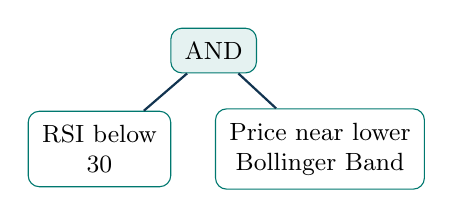
\begin{tikzpicture}[box/.style={draw=accent,rounded corners,align=center,inner sep=5pt,font=\small},edge/.style={draw=navy,thick}]
\node[box,fill=accent!10] (both) at (0,0) {AND};
\node[box] (rsi) at (-1.45,-1.25) {RSI below\\30};
\node[box] (band) at (1.35,-1.25) {Price near lower\\Bollinger Band};
\draw[edge] (both) -- (rsi);
\draw[edge] (both) -- (band);
\end{tikzpicture}
\par\smallskip{\small Both conditions must hold for this rule to signal entry.}
\end{column}
\begin{column}{.49\textwidth}
\textbf{How the search works}
\begin{itemize}
\item Start with 40 candidate rule trees.
\item Select better-scoring parents, swap branches between trees, and mutate individual trees.
\item Evolve the population for 12 generations. A penalty per node favors shorter rules.
\end{itemize}
\end{column}
\end{columns}
\key{The evolved rule supplies one of five signals to the final equity trading policy.}
\end{frame}

\begin{frame}{From single-stock rules to a shared portfolio}
\key{Search for entries and exits}
Test VWAP, RSI and Bollinger mean reversion alongside Donchian breakouts. Vary stops and profit targets.
\key{Freeze the rule before evaluation}
The default walk-forward schedule fits six prior calendar months, trades the selected rule for one month, then advances one month.
\key{Replay one account}
Rank stocks monthly using trailing performance. Admit the top 10 or 20 and draw each entry from the same pool of capital.
\end{frame}

\begin{frame}{India's top 10 finished ahead of buy-and-hold}
\pair{10-portfolio_value.png}{December 2020--August 2025}{Top 10 returned \textbf{250.87\%}, versus \textbf{220.97\%} for equal-money buy-and-hold. Maximum daily drawdown was 19.83\%.\\[2mm]
Top 20 returned 104.85\% with a 24.73\% drawdown. Allocation per entry also differed: 12\% for top 10 and 10\% for top 20.}
\end{frame}

\begin{frame}{US stocks: the top-20 GA/GP portfolio}
\centering
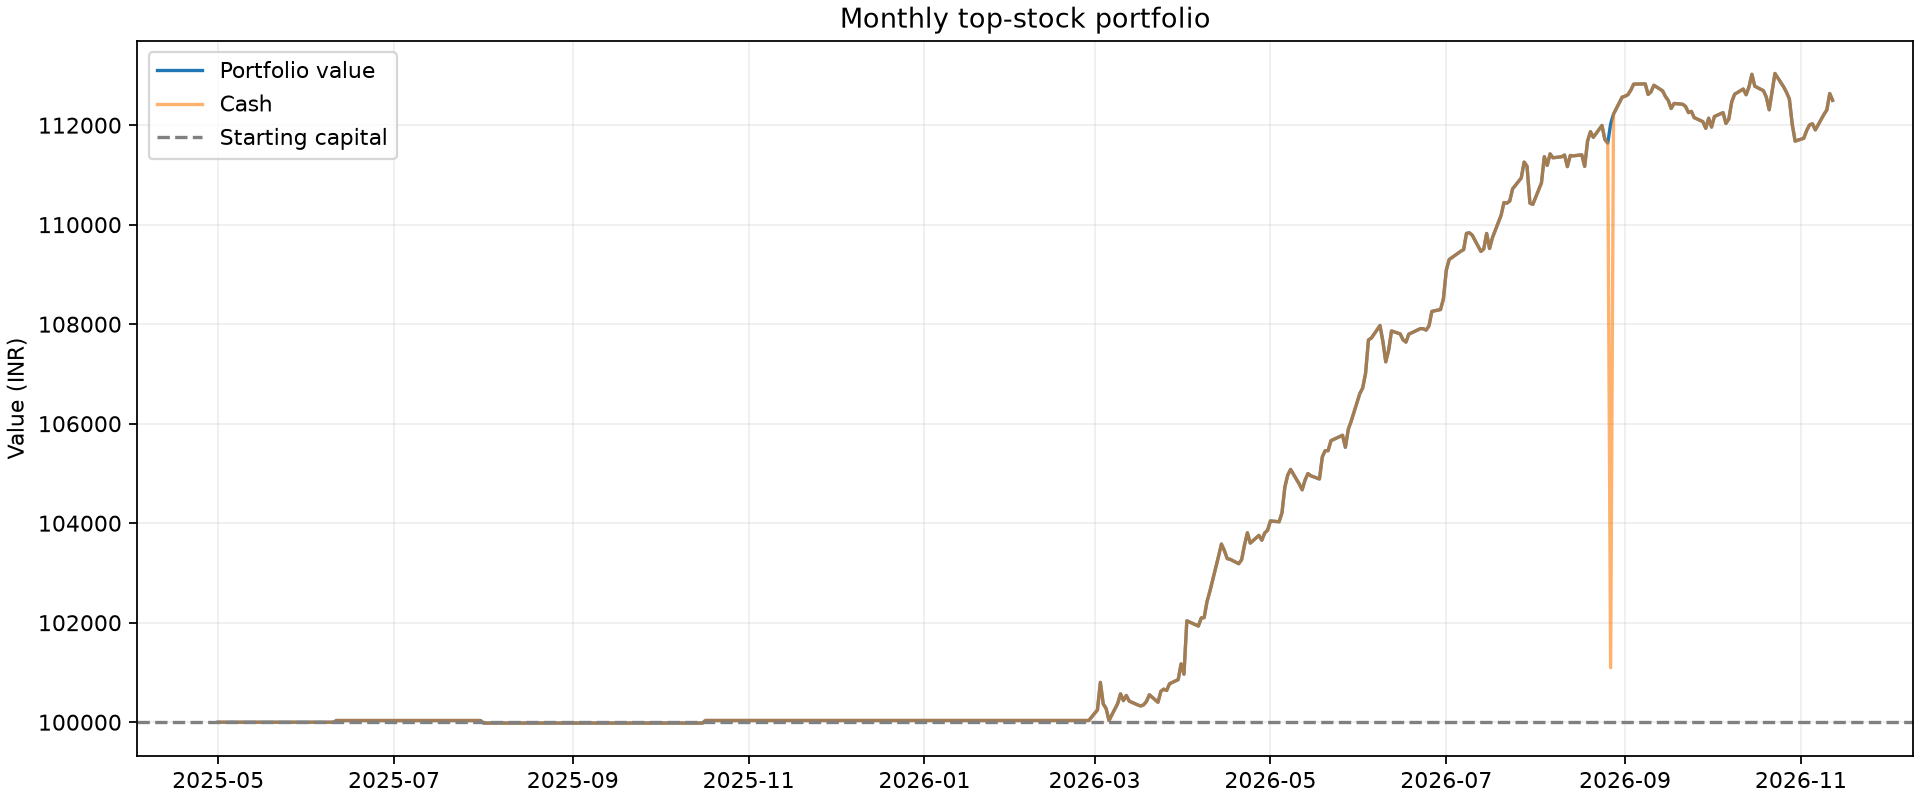
\includegraphics[width=\linewidth,height=5.55cm,keepaspectratio]{11-portfolio_value.png}
\par\smallskip{\small 1 May 2025--12 November 2026 \qquad USD 100,000 to USD 112,499.25 \qquad \textbf{+12.50\%}}
\end{frame}

\begin{frame}{US portfolios traded sparsely and trailed holding}
\pair{monthly-us.png}{May 2025--November 2026}{Top 10 gained \textbf{8.92\%} and top 20 gained \textbf{12.50\%}. Equal-money buy-and-hold gained \textbf{40.97\%}.\\[2mm]
Only one stock had a trailing score before March 2026. Even over the active period, top 20 gained 12.46\% against 13.28\% for holding.}
\end{frame}

\begin{frame}{Fees absorbed over half of India's top-10 trading profit}
\centering
\begin{tabular}{lrr}\toprule
Recorded top-10 portfolio measure & India (INR) & US (USD)\\\midrule
Profit before recorded fees & 5,928,109 & 10,200\\
Explicit fees & 3,419,384 & 1,277\\
Profit after recorded fees & 2,508,725 & 8,923\\
Share of pre-fee profit consumed & 57.68\% & 12.52\%\\\bottomrule
\end{tabular}
\par\bigskip\raggedright Covering explicit charges required about \textbf{5.21 basis points} per round trip in India and \textbf{0.29} in the US replay under its zero-commission assumption.
\end{frame}

\begin{frame}{A drawdown-aware policy gained 4.02\% on held-out data}
\pair{12-equity.png}{US intraday strategy signals}{An advantage actor--critic policy used the four technical strategy signals and the evolved entry rule. Its reward combined equity growth with a penalty for increases in drawdown.\\[2mm]
From 1 September to 12 November 2026, the policy recorded \textbf{1.38\% maximum drawdown}, 1,040 fills and USD 57.03 in fees.}
\end{frame}

\begin{frame}{What the experiments establish}
\key{Forecasting}
USD/INR's 55.51\% directional accuracy translated into three extra correct days over always-up. A repeated-seed comparison with standard squared error would isolate the contribution of loss design.
\key{Execution}
EUR/USD earned a positive return with more losses than wins. Finer price data would help test which stops and targets could actually have filled.
\key{Portfolio performance}
The Indian top 10 beat holding after recorded fees. Both US portfolios trailed their benchmark. Testing on new periods with matched exposure would help distinguish signal quality from time spent invested.
\end{frame}
\appendix
{\setbeamertemplate{background}{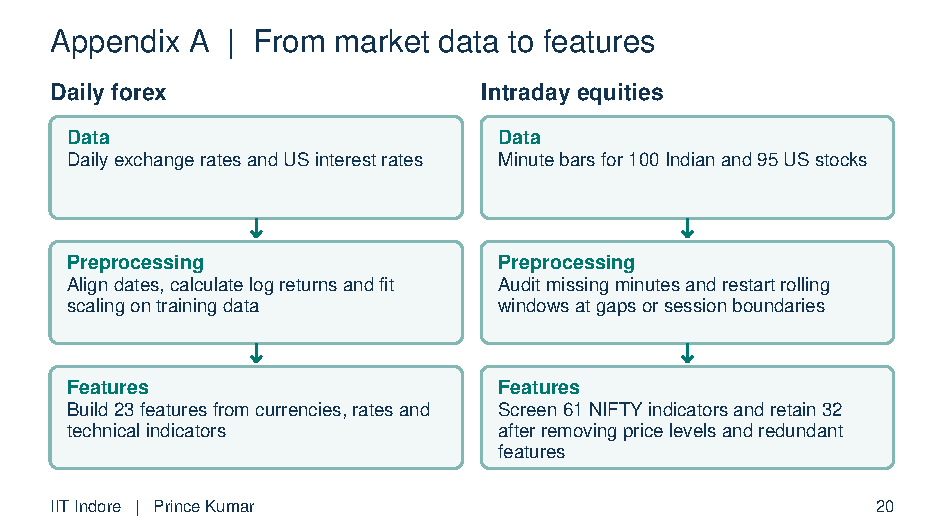
\includegraphics[width=\paperwidth,height=\paperheight]{appendix-features.pdf}}
\begin{frame}[plain]\null\end{frame}
}
{\setbeamertemplate{background}{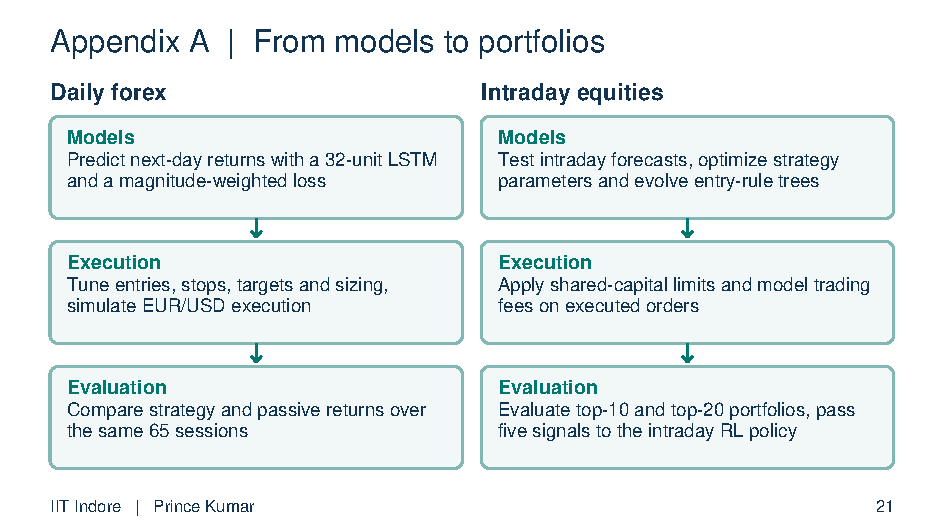
\includegraphics[width=\paperwidth,height=\paperheight]{appendix-models.pdf}}
\begin{frame}[plain]\null\end{frame}
}
{\setbeamertemplate{background}{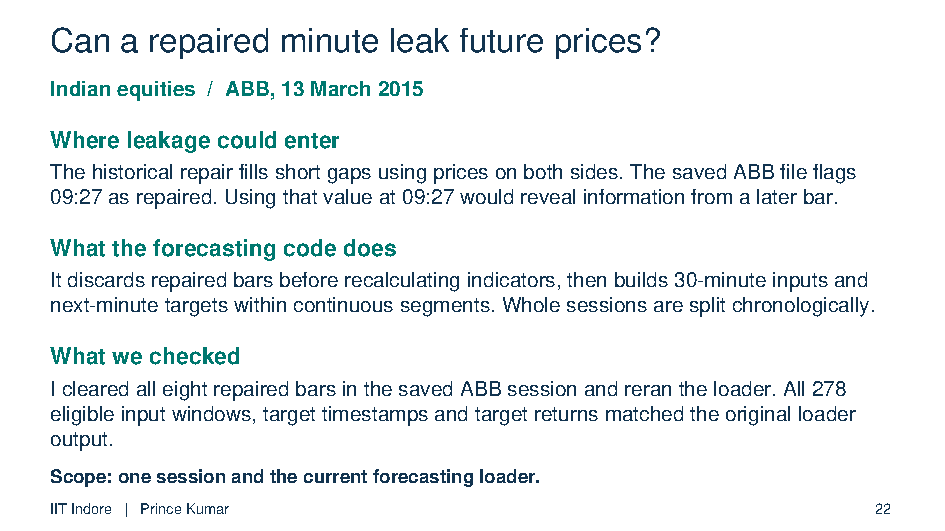
\includegraphics[width=\paperwidth,height=\paperheight]{equity-preprocessing.pdf}}
\begin{frame}[plain]\null\end{frame}
}
\end{document}
